% !Mode:: "TeX:UTF-8"
% !TEX program = xelatex

%%%%%%%%%% Port for macOS %%%%%%%%%%%
% Modified: Qin Yubo

\def\usewhat{xelatex}
\documentclass[12pt,openany,oneside,AutoFakeBold]{ctexbook}
                                           % 本科生毕业论文通常采用单页排版
% !Mode:: "TeX:UTF-8"
%  Authors: 张井   Jing Zhang: prayever@gmail.com     天津大学2010级管理与经济学部信息管理与信息系统专业硕士生
%           余蓝涛 Lantao Yu: lantaoyu1991@gmail.com  天津大学2008级精密仪器与光电子工程学院测控技术与仪器专业本科生

%%%%%%%%%% Package %%%%%%%%%%%%
\usepackage{CJK}
\usepackage{pdfpages}

\usepackage{lastpage}
\usepackage{lmodern}
\usepackage[T1]{fontenc}
\usepackage{graphicx}                       % 支持插图处理
\usepackage[a4paper,text={146.4true mm,239.2 true mm},top= 26.2true mm,left=31.8 true mm,head=6true mm,headsep=6.5true mm,foot=16.5true mm]{geometry}
                                            % 支持版面尺寸设置
\usepackage[squaren]{SIunits}               % 支持国际标准单位

\usepackage{titlesec}                       % 控制标题的宏包
\usepackage{titletoc}                       % 控制目录的宏包
\usepackage{fancyhdr}                       % fancyhdr宏包 支持页眉和页脚的相关定义
%\usepackage{ctex}                     % 支持中文显示
\usepackage{CJKpunct}                       % 精细调整中文的标点符号
\usepackage{color}                          % 支持彩色
\usepackage{amsmath}                        % AMSLaTeX宏包 用来排出更加漂亮的公式
\usepackage{amssymb}                        % 数学符号生成命令
\usepackage[below]{placeins}    %允许上一个section的浮动图形出现在下一个section的开始部分,还提供\FloatBarrier命令,使所有未处理的浮动图形立即被处理
\usepackage{multirow}                       % 使用Multirow宏包,使得表格可以合并多个row格
\usepackage{booktabs}                       % 表格,横的粗线;\specialrule{1pt}{0pt}{0pt}
\usepackage{longtable}                      % 支持跨页的表格。
\usepackage{tabularx}                       % 自动设置表格的列宽
\usepackage{subfigure}                      % 支持子图 %centerlast 设置最后一行是否居中
\usepackage[subfigure]{ccaption}            % 支持子图的中文标题
\usepackage[sort&compress,numbers]{natbib}  % 支持引用缩写的宏包
\usepackage{enumitem}                       % 使用enumitem宏包,改变列表项的格式
\usepackage{calc}                           % 长度可以用+ - * / 进行计算
\usepackage{txfonts}                        % 字体宏包
\usepackage{bm}                             % 处理数学公式中的黑斜体的宏包
\usepackage[amsmath,thmmarks,hyperref]{ntheorem}  % 定理类环境宏包,其中 amsmath 选项用来兼容 AMS LaTeX 的宏包
\usepackage{CJKnumb}                        % 提供将阿拉伯数字转换成中文数字的命令
\usepackage{indentfirst}                    % 首行缩进宏包
\usepackage{CJKutf8}                        % 用在UTF8编码环境下,它可以自动调用CJK,同时针对UTF8编码作了设置
%\usepackage{hypbmsec}                      % 用来控制书签中标题显示内容
\newcommand{\tabincell}[2]{\begin{tabular}{@{}#1@{}}#2\end{tabular}}
\usepackage{xcolor}
%支持代码环境
\usepackage{listings}
\usepackage{mhchem}
\usepackage{geometry}
\lstset{numbers=left,
language=[ANSI]{C},
numberstyle=\tiny,
extendedchars=false,
showstringspaces=false,
breakatwhitespace=false,
breaklines=true,
captionpos=b,
keywordstyle=\color{blue!70},
commentstyle=\color{red!50!green!50!blue!50},
frame=shadowbox,
rulesepcolor=\color{red!20!green!20!blue!20}
}
%支持算法环境
\usepackage[boxed,ruled,lined]{algorithm2e}
\usepackage{algorithmic}

\usepackage{array}
\newcommand{\PreserveBackslash}[1]{\let\temp=\\#1\let\\=\temp}
\newcolumntype{C}[1]{>{\PreserveBackslash\centering}p{#1}}
\newcolumntype{R}[1]{>{\PreserveBackslash\raggedleft}p{#1}}
\newcolumntype{L}[1]{>{\PreserveBackslash\raggedright}p{#1}}

\def\atemp{xelatex}\ifx\atemp\usewhat
\usepackage[unicode,
            pdfstartview=FitH,
            bookmarksnumbered=true,
            bookmarksopen=true,
            colorlinks=false,
            pdfborder={0 0 1},
            citecolor=blue,
            linkcolor=red,
            anchorcolor=green,
            urlcolor=blue,
            breaklinks=true
            ]{hyperref}
\fi
\usepackage{hyperref}
\hypersetup{
    hidelinks,
    colorlinks=true,
    linkcolor=black,
    citecolor=black,
    urlcolor=black,
    }
                                % 定义本文所使用宏包
\graphicspath{{figures/}}                            % 定义所有的图像文件在 figures 子目录下
\geometry{a4paper,left=3.57cm,right=2.77cm,top=2.75cm,bottom=2.54cm,footskip=6.4mm,headheight=4.5mm,headsep=6.1mm}  
\begin{document}                                     % 开始全文
% !Mode:: "TeX:UTF-8"
%  Authors: 张井   Jing Zhang: prayever@gmail.com     天津大学2010级管理与经济学部信息管理与信息系统专业硕士生
%           余蓝涛 Lantao Yu: lantaoyu1991@gmail.com  天津大学2008级精密仪器与光电子工程学院测控技术与仪器专业本科生

%%%%%%%%%%%%%%%%% Fonts Definition and Basics %%%%%%%%%%%%%%%%%
%\newcommand{\song}{\CJKfamily{song}}    % 宋体
%\newcommand{\fs}{\CJKfamily{fs}}        % 仿宋体
%\newcommand{\kai}{\CJKfamily{kai}}      % 楷体
%\newcommand{\hei}{\CJKfamily{hei}}      % 黑体
%\newcommand{\li}{\CJKfamily{li}}        % 隶书
\newcommand{\song}{\songti}    % 宋体
\newcommand{\fs}{\fangsong}        % 仿宋体
\newcommand{\kai}{\kaishu}      % 楷体
\newcommand{\hei}{\heiti}      % 黑体
\newcommand{\li}{\lishu}        % 隶书
\newcommand{\yihao}{\fontsize{26pt}{26pt}\selectfont}       % 一号, 单倍行距
\newcommand{\xiaoyi}{\fontsize{24pt}{24pt}\selectfont}      % 小一, 单倍行距
\newcommand{\erhao}{\fontsize{22pt}{1.25\baselineskip}\selectfont}       % 二号, 1.25倍行距
\newcommand{\xiaoer}{\fontsize{18pt}{18pt}\selectfont}      % 小二, 单倍行距
\newcommand{\sanhao}{\fontsize{16pt}{16pt}\selectfont}      % 三号, 单倍行距
\newcommand{\xiaosan}{\fontsize{15pt}{15pt}\selectfont}     % 小三, 单倍行距
\newcommand{\sihao}{\fontsize{14pt}{14pt}\selectfont}       % 四号, 单倍行距
\newcommand{\xiaosi}{\fontsize{12pt}{12pt}\selectfont}      % 小四, 单倍行距
\newcommand{\wuhao}{\fontsize{10.5pt}{10.5pt}\selectfont}   % 五号, 单倍行距
\newcommand{\xiaowu}{\fontsize{9pt}{9pt}\selectfont}        % 小五, 单倍行距

%\CJKtilde  % 重新定义了波浪符~的意义
% JUST DON'T USE CJK
% 使用 ctexbook 之后已无必要
\newcommand\prechaptername{第}
\newcommand\postchaptername{章}

\punctstyle{hangmobanjiao}             % 调整中文字符的表示,行内占一个字符宽度,行尾占半个字符宽度

% 调整罗列环境的布局
\setitemize{leftmargin=3em,itemsep=0em,partopsep=0em,parsep=0em,topsep=-0em}
\setenumerate{leftmargin=3em,itemsep=0em,partopsep=0em,parsep=0em,topsep=0em}

% 避免宏包 hyperref 和 arydshln 不兼容带来的目录链接失效的问题。
\def\temp{\relax}
\let\temp\addcontentsline
\gdef\addcontentsline{\phantomsection\temp}

% 自定义项目列表标签及格式 \begin{publist} 列表项 \end{publist}
\newcounter{pubctr} %自定义新计数器
\newenvironment{publist}{%%%%%定义新环境
\begin{list}{[\arabic{pubctr}]} %%标签格式
    {
     \usecounter{pubctr}
     \setlength{\leftmargin}{2.5em}   % 左边界 \leftmargin =\itemindent + \labelwidth + \labelsep
     \setlength{\itemindent}{0em}     % 标号缩进量
     \setlength{\labelsep}{1em}       % 标号和列表项之间的距离,默认0.5em
     \setlength{\rightmargin}{0em}    % 右边界
     \setlength{\topsep}{0ex}         % 列表到上下文的垂直距离
     \setlength{\parsep}{0ex}         % 段落间距
     \setlength{\itemsep}{0ex}        % 标签间距
     \setlength{\listparindent}{0pt}  % 段落缩进量
    }}
{\end{list}}

\makeatletter
\renewcommand\normalsize{
  \@setfontsize\normalsize{12pt}{12pt} % 小四对应 12 pt
  \setlength\abovedisplayskip{4pt}
  \setlength\abovedisplayshortskip{4pt}
  \setlength\belowdisplayskip{\abovedisplayskip}
  \setlength\belowdisplayshortskip{\abovedisplayshortskip}
  \let\@listi\@listI}
\def\defaultfont{\renewcommand{\baselinestretch}{1.63}\normalsize\selectfont} % 设置行距

\renewcommand{\CJKglue}{\hskip -0.1 pt plus 0.08\baselineskip} % 控制字间距,使每行 34 个汉字
\makeatother

%%%%%%%%%%%%% Contents %%%%%%%%%%%%%%%%%
\renewcommand{\contentsname}{目\quad 录}
\setcounter{tocdepth}{2} % 控制目录深度
% 使用 ctexbook 之后已无必要
%\titlecontents{chapter}[2em]{\vspace{.5\baselineskip}\xiaosan\song}
             %{\prechaptername\CJKnumber{\thecontentslabel}\postchaptername\qquad}{}
             %{\hspace{.5em}\titlerule*[10pt]{$\cdot$}\sihao\contentspage}
\titlecontents{chapter}[2em]{\vspace{.1\baselineskip}\sihao\song}
             {{\heiti \thecontentslabel\quad}}{}
             {\hspace{.5em}\titlerule*[10pt]{$...$}\sihao{\song\contentspage}}
\titlecontents{section}[3em]{\vspace{.1\baselineskip}\sihao\song}
             {\quad{{{\thecontentslabel}}\quad}}{}
             {\hspace{.5em}\titlerule*[10pt]{$...$}\sihao{\song\contentspage}}
\titlecontents{subsection}[4em]{\song\vspace{.1\baselineskip}\sihao\song}
             {\,\quad{{\thecontentslabel}\quad}}{}
             {\hspace{.5em}\titlerule*[10pt]{$...$}\sihao{\song\contentspage}}

%%%%%%%%%% Chapter and Section %%%%%%%%%%%%%
\setcounter{secnumdepth}{4}
\setlength{\parindent}{2em}
\renewcommand{\chaptername}{\prechaptername\CJKnumber{\thechapter}\postchaptername}
\titleformat{\chapter}{\centering\xiaosan\song}{\hei\chaptername}{2em}{}
\titlespacing{\chapter}{0pt}{0.1\baselineskip}{0.8\baselineskip}
\titleformat{\section}{\sihao\sf\hei}{\thesection}{1em}{}
\titlespacing{\section}{0pt}{0.15\baselineskip}{0.25\baselineskip}
\titleformat{\subsection}{\sihao\sf\hei}{{\thesubsection}}{1em}{}
\titlespacing{\subsection}{0pt}{0.1\baselineskip}{0.3\baselineskip}
\titleformat{\subsubsection}{\sihao\sf\hei}{{\thesubsubsection}}{1em}{}
\titlespacing{\subsubsection}{0pt}{0.05\baselineskip}{0.1\baselineskip}

%%%%%%%%%% Table, Figure and Equation %%%%%%%%%%%%%%%%%
\renewcommand{\tablename}{表}                                     % 插表题头
\renewcommand{\figurename}{图}                                    % 插图题头
\renewcommand{\thefigure}{\arabic{chapter}-\arabic{figure}}       % 使图编号为 7-1 的格式 %\protect{~}
\renewcommand{\thesubfigure}{\alph{subfigure})}                   % 使子图编号为 a) 的格式
\renewcommand{\thesubtable}{(\alph{subtable})}                    % 使子表编号为 (a) 的格式
\renewcommand{\thetable}{\arabic{chapter}-\arabic{table}}         % 使表编号为 7-1 的格式
\renewcommand{\theequation}{\arabic{chapter}-\arabic{equation}}   % 使公式编号为 7-1 的格式
\newcommand{\ud}{\mathrm{d}}

%%%%%% 定制浮动图形和表格标题样式 %%%%%%
\makeatletter
\long\def\@makecaption#1#2{
   \vskip\abovecaptionskip
   \sbox\@tempboxa{\centering\wuhao\song{#1\qquad #2} }
   \ifdim \wd\@tempboxa >\hsize
     \centering\wuhao\song{#1\quad #2} \par
   \else
     \global \@minipagefalse
     \hb@xt@\hsize{\hfil\box\@tempboxa\hfil}
   \fi
   \vskip\belowcaptionskip}
\makeatother
\captiondelim{~~~~} %用来控制longtable表头分隔符

%%%%%%%%%% Theorem Environment %%%%%%%%%%%%%%%%%
\theoremstyle{plain}
\theorembodyfont{\song\rmfamily}
\theoremheaderfont{\hei\rmfamily}
\newtheorem{theorem}{定理~}[chapter]
\newtheorem{lemma}{引理~}[chapter]
\newtheorem{axiom}{公理~}[chapter]
\newtheorem{proposition}{命题~}[chapter]
\newtheorem{prop}{性质~}[chapter]
\newtheorem{corollary}{推论~}[chapter]
\newtheorem{definition}{定义~}[chapter]
\newtheorem{conjecture}{猜想~}[chapter]
\newtheorem{example}{例~}[chapter]
\newtheorem{remark}{注~}[chapter]
%\newtheorem{algorithm}{算法~}[chapter]
\newenvironment{proof}{\noindent{\hei 证明:}}{\hfill $ \square $ \vskip 4mm}
\theoremsymbol{$\square$}

%%%%%%%%%% Page: number, header and footer  %%%%%%%%%%%%%%%%%

%\frontmatter 或 \pagenumbering{roman}
%\mainmatter 或 \pagenumbering{arabic}
\makeatletter
\renewcommand\frontmatter{\clearpage
  \@mainmatterfalse
  }
\makeatother

%%%%%%%%%%% Code: Listings from MCM Template %%%%%%%%%%%%

\definecolor{grey}{rgb}{0.8,0.8,0.8}
\definecolor{darkgreen}{rgb}{0,0.3,0}
\definecolor{darkblue}{rgb}{0,0,0.3}
\def\lstbasicfont{\fontfamily{pcr}\selectfont\footnotesize}
\lstset{%
% indexing
   % numbers=left,
   % numberstyle=\small,%
% character display
    showstringspaces=false,
    showspaces=false,%
    tabsize=4,%
% style
    frame=lines,%
    basicstyle={\footnotesize\lstbasicfont},%
    keywordstyle=\color{darkblue}\bfseries,%
    identifierstyle=,%
    commentstyle=\color{darkgreen},%\itshape,%
    stringstyle=\color{black}%
}
\lstloadlanguages{C,C++,Java,Matlab,Mathematica,Python}

%%%%%%%%%%%% References %%%%%%%%%%%%%%%%%
\renewcommand{\bibname}{{\begin{center} \xiaosan 参考文献\end{center}}}
% 重定义参考文献样式,来自thu
\makeatletter
\renewenvironment{thebibliography}[1]{
    \titleformat{\chapter}{\raggedright\sihao\hei}{\chaptername}{2em}{}
   \chapter*{\bibname}
   \wuhao
   \list{\@biblabel{\@arabic\c@enumiv}}
        {\renewcommand{\makelabel}[1]{##1\hfill}
         \settowidth\labelwidth{0 cm}
         \setlength{\labelsep}{0pt}
         \setlength{\itemindent}{0pt}
         \setlength{\leftmargin}{\labelwidth+\labelsep}
         \addtolength{\itemsep}{-0.7em}
         \usecounter{enumiv}
         \let\p@enumiv\@empty
         \renewcommand\theenumiv{\@arabic\c@enumiv}}
    \sloppy\frenchspacing
    \clubpenalty4000
    \@clubpenalty \clubpenalty
    \widowpenalty4000
    \interlinepenalty4000
    \sfcode`\.\@m}
   {\def\@noitemerr
     {\@latex@warning{Empty `thebibliography' environment}}
    \endlist\frenchspacing}
\makeatother

\addtolength{\bibsep}{-0.5em}     % 缩小参考文献间的垂直间距
\setlength{\bibhang}{2em}         % 每个条目自第二行起缩进的距离

% 参考文献引用作为上标出现
%\newcommand{\citeup}[1]{\textsuperscript{\cite{#1}}}
\makeatletter
    \def\@cite#1#2{\textsuperscript{[{#1\if@tempswa , #2\fi}]}}
\makeatother
%% 引用格式
\bibpunct{[}{]}{,}{s}{}{,}

%%%%%%%%%%%% Cover %%%%%%%%%%%%%%%%%
% 封面、摘要、版权、致谢格式定义
\makeatletter
\def\ctitle#1{\def\@ctitle{#1}}\def\@ctitle{}
\def\cdegree#1{\def\@cdegree{#1}}\def\@cdegree{}
\def\caffil#1{\def\@caffil{#1}}\def\@caffil{}
\def\csubject#1{\def\@csubject{#1}}\def\@csubject{}
\def\cgrade#1{\def\@cgrade{#1}}\def\@cgrade{}
\def\cauthor#1{\def\@cauthor{#1}}\def\@cauthor{}
\def\cnumber#1{\def\@cnumber{#1}}\def\@cnumber{}
\def\csupervisor#1{\def\@csupervisor{#1}}\def\@csupervisor{}
\def\crank#1{\def\@crank{#1}}\def\@crank{}
\def\cdate#1{\def\@cdate{#1}}\def\@cdate{}
\long\def\cabstract#1{\long\def\@cabstract{#1}}\long\def\@cabstract{}
\long\def\eabstract#1{\long\def\@eabstract{#1}}\long\def\@eabstract{}
\def\ckeywords#1{\def\@ckeywords{#1}}\def\@ckeywords{}
\def\ekeywords#1{\def\@ekeywords{#1}}\def\@ekeywords{}
\def\cheading#1{\def\@cheading{#1}}\def\@cheading{}


\pagestyle{fancy}
  \fancyhf{}
  \fancyhead[C]{\song\wuhao \@cheading}  % 页眉显示天津大学 20XX 届本科生毕业论文
  \fancyfoot[C]{\song\xiaowu ~\thepage~}
\newlength{\@title@width}

%\setlength{\voffset}{-12.5mm} % 页眉距边距15.0 = 27.5(上边距)-12.5
%\setlength{\footskip}{-9.9mm} % 页脚距边距17.5 = 25.4(下边距)-9.9
% 定义封面
\def\makecover{
%\cleardoublepage%
   \phantomsection
    \pdfbookmark[-1]{\@ctitle}{ctitle}

    \begin{titlepage}
      \vspace*{31.5pt}
      \begin{center}

  \begin{figure}[h]
  \centering
  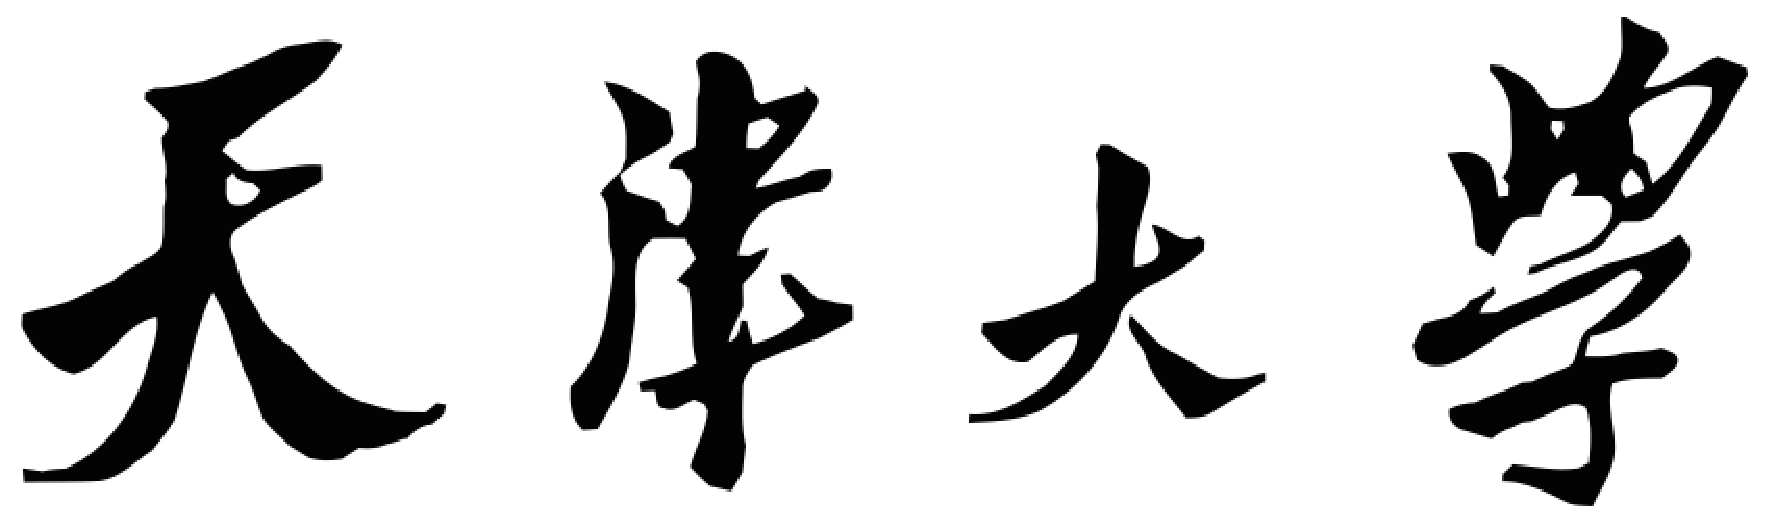
\includegraphics[width=0.4\textwidth]{figures/tjuname.eps}
  \end{figure}
  \vspace*{21pt}
  \erhao{\hei\textbf{本科生毕业论文}}
  \vspace*{52.5pt}

  \begin{figure}[h]
  \centering
  
\includegraphics[width=0.3\textwidth]{figures/tjulogo.eps}
  \end{figure}

  \vspace*{5pt}
  \sanhao{\hei\textbf{题目:\@ctitle}}
  \vspace*{16pt}
  
  \vspace*{24pt}
  \renewcommand\arraystretch{1.5}
  \setlength{\@title@width}{5cm}
  {\fontsize{16pt}{16pt}\songti {\textbf{
  \begin{tabular}{lc} 
    学\qquad 院&  \underline{\makebox[\@title@width][c]{\@caffil}} \\
    专\qquad 业 &  \underline{\makebox[\@title@width][c]{\@csubject}} \\
    年\qquad 级  &  \underline{\makebox[\@title@width][c]{\@cgrade}}\\
    姓\qquad 名 &  \underline{\makebox[\@title@width][c]{\@cauthor}} \\
    学\qquad 号 &  \underline{\makebox[\@title@width][c]{\@cnumber}} \\
    指导教师 &  \underline{\makebox[\@title@width][c]{\@csupervisor}} \\
  \end{tabular}}}
 }
  \vspace*{21pt}

%\song\sanhao{\textbf{\@cdate}}
\end{center}
\end{titlepage}
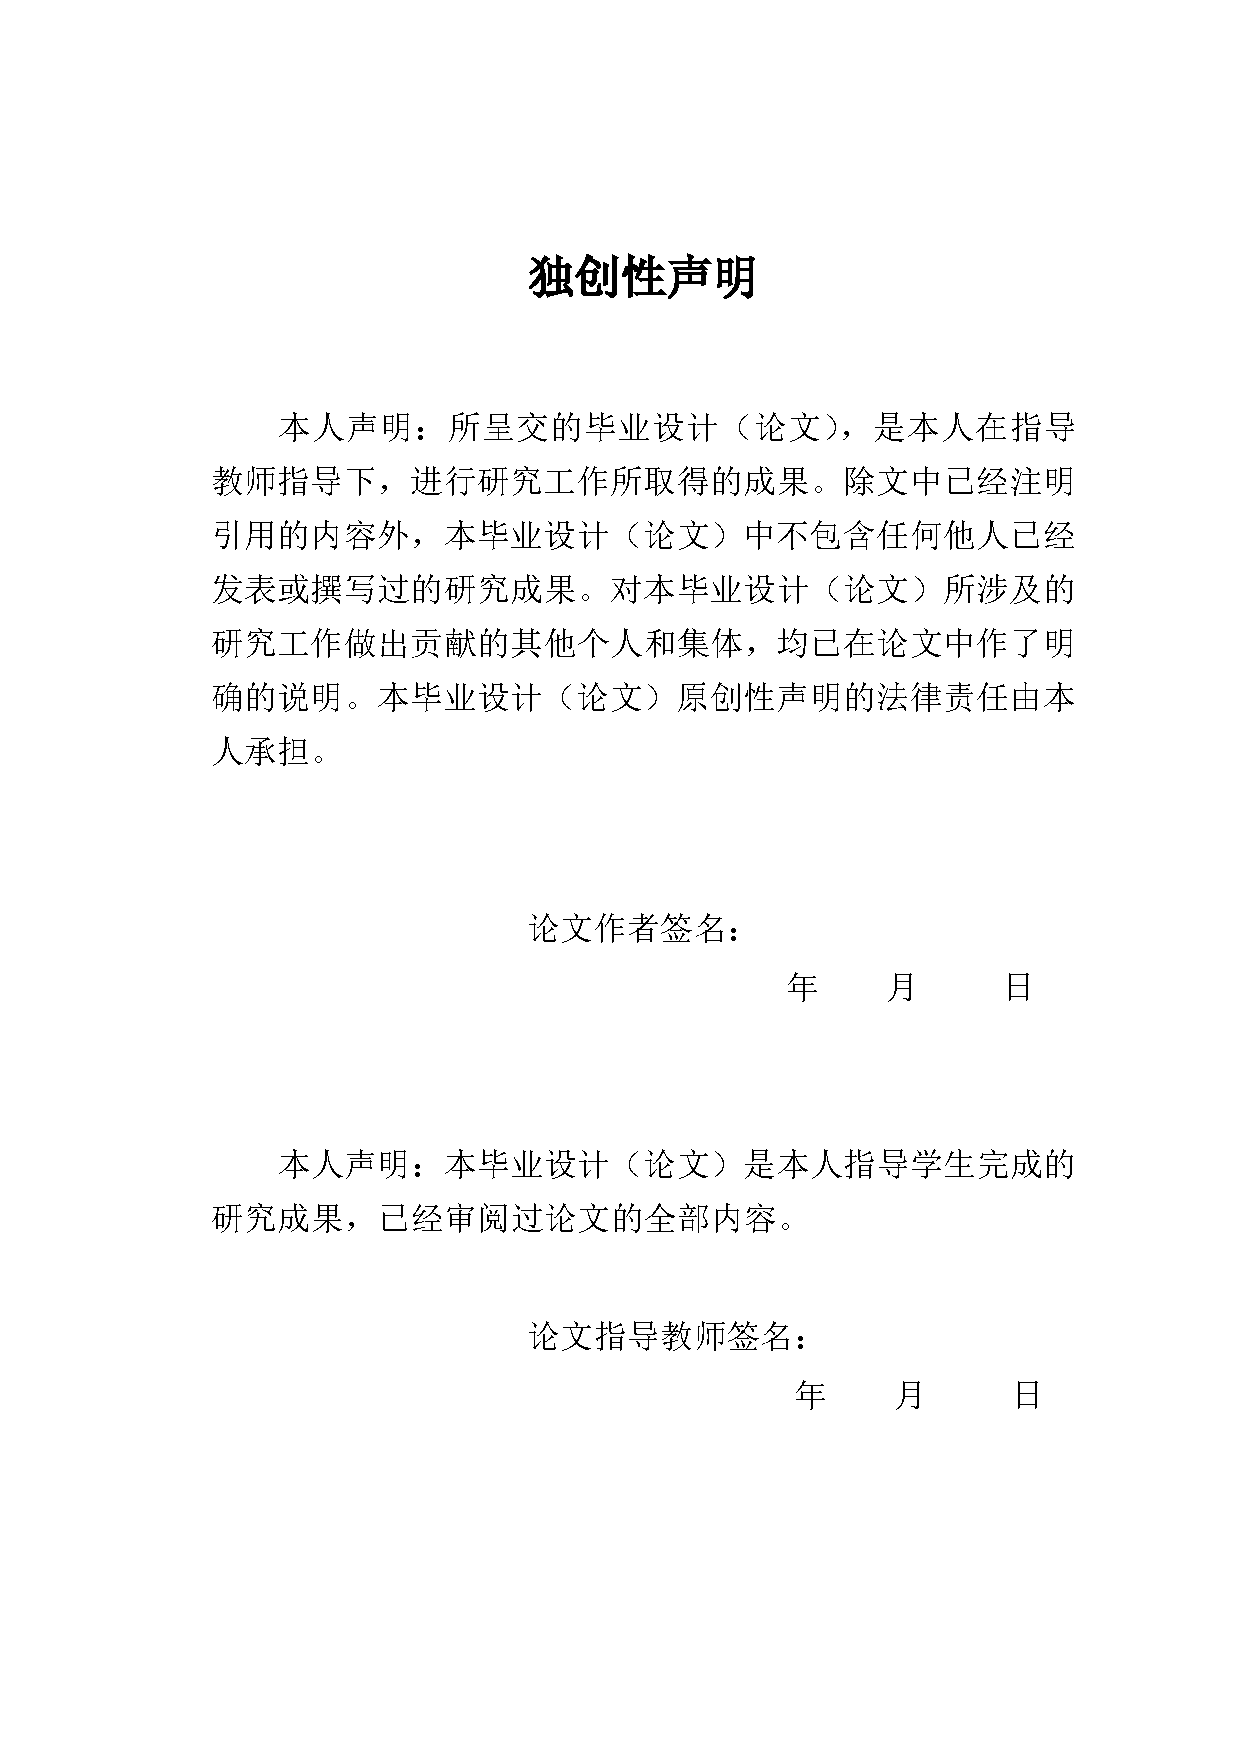
\includepdf{独创性声明.pdf}
%%%%%%%%%%%%%%%%%%%   Abstract and Keywords  %%%%%%%%%%%%%%%%%%%%%%%
\clearpage
\setcounter{page}{1}    
\pagenumbering{Roman}
\markboth{摘~要}{摘~要}
\pdfbookmark[0]{摘~~要}{cabstract}
%\addcontentsline{toc}{chapter}{摘~要}
%\chapter*{\centering\sanhao\hei\bfseries 摘\qquad 要}
\chapter*{\centering\erhao\songti \textbf{摘\quad 要}}
\song\defaultfont
\@cabstract
\vspace{\baselineskip}

\hangafter=1\hangindent=52.3pt\noindent
{\hei\xiaosi 关键词:} \@ckeywords
%\thispagestyle{empty}

%%%%%%%%%%%%%%%%%%%   English Abstract  %%%%%%%%%%%%%%%%%%%%%%%%%%%%%%
\clearpage
%\phantomsection
\markboth{ABSTRACT}{ABSTRACT}
\pdfbookmark[0]{ABSTRACT}{eabstract}
%\addcontentsline{toc}{chapter}{ABSTRACT}
\chapter*{\centering\erhao{\bf{ABSTRACT}}}
%\vspace{\baselineskip}
\@eabstract
\vspace{\baselineskip}

\hangafter=1\hangindent=60pt\noindent
{\textbf{Keywords:}} \@ekeywords
%\thispagestyle{empty}
}
\makeatother
                                 % 完成对论文各个部分格式的设置
\frontmatter                                         % 以下是论文导言部分,包括论文的封面,中英文摘要和中文目录
\fancypagestyle{plain}{
\fancyhf{}
\renewcommand{\headrulewidth}{0 pt}
\fancyfoot[C]{\song\xiaowu~\thepage~}
}
% 直接从 Word 模板生成封面导出 pdf 似乎更方便
% !Mode:: "TeX:UTF-8"

%%  可通过增加或减少 setup/format.tex中的
%%  第274行 \setlength{\@title@width}{8cm}中 8cm 这个参数来 控制封面中下划线的长度。

\cheading{天津大学~2024~届本科生毕业论文}      % 设置正文的页眉,需要填上对应的毕业年份
\ctitle{有机场效应晶体管}    % 封面用论文标题,自己可手动断行
\caffil{化工学院} % 学院名称
\csubject{分子科学与工程}   % 专业名称
\cgrade{2020~级}            % 年级
\cauthor{张三}            % 学生姓名
\cnumber{3020207000}        % 学生学号
\csupervisor{王五}        % 导师姓名
\crank{副教授}              % 导师职称

\cdate{\the\year~年~\the\month~月~\the\day~日}

\cabstract{中文摘要}

\ckeywords{关键词1;关键词2}

\eabstract{
English Abstract}

\ekeywords{keyWords1, keyWords2}

\makecover

\clearpage
                                % 封面

%%%%%%%%%%   目录   %%%%%%%%%%
\defaultfont
\clearpage{\pagestyle{empty}\cleardoublepage}
\setcounter{page}{1}                                 % 单独从 1 开始编页码
\pagenumbering{arabic}
\titleformat{\chapter}{\centering\sanhao\hei}{\chaptername}{2em}{} % 设置目录两字的格式
\pdfbookmark[0]{目~~录}{mulu}
\tableofcontents                                     % 中文目录
\fancypagestyle{plain}{
\fancyhf{}
\renewcommand{\headrulewidth}{0 pt}
\fancyfoot[C]{\song\xiaowu~\thepage~}
}
\thispagestyle{plain}

\mainmatter\defaultfont\sloppy\raggedbottom
\makeatletter
\fancypagestyle{plain}{                              % 设置开章页眉页脚风格
    \fancyhf{}
    \fancyhead[C]{\song\wuhao \@cheading}            % 首页页眉格式
    \fancyfoot[C]{\song\xiaowu ~\thepage~}           % 首页页脚格式
    \renewcommand{\headrulewidth}{0.5pt}
    \renewcommand{\footrulewidth}{0pt}
}
\makeatother
\setcounter{page}{1}                                 % 单独从 1 开始编页码
\titleformat{\chapter}{\centering\xiaosan\hei}{\chaptername}{2em}{} % 恢复chapter标题格式要求

%%%%%%%%%  正文  %%%%%%%%%
% !Mode:: "TeX:UTF-8"
% !TEX root = tjumain.tex

\iffalse
\bibliography{reference/reference.bib} % 欺骗latextools获取bib文件
\fi

%%%%%%% 正文 %%%%%%%

%%%% 引言 %%%%
\chapter{引言}
上世纪七十年代,“导电聚合物”的发现震惊了世界\cite{PhysRevLett.40.1472}。

\chapter{理论与计算方法}
\vspace{2mm}
\section{电子结构理论}
\vspace{2mm}
\vspace{2mm}
\subsection{Schrödinger方程和Born-Oppenheimer近似}
\vspace{2mm}
量子力学假设,微观粒子所处的状态可用波函数$\psi({\bf r},t)$进行表示,微观粒子在空间中分布的概率密度可用波函数的平方$|\psi({\bf r},t)|^2=\psi^*\psi$表示,波函数的时间演化遵循Schrödinger方程,Schrödinger方程的一般形式为\vspace{3mm}
\begin{equation}
    \label{eqn:sch_t}
\hat H \psi ({\bf r},t)=i\hbar\frac{\partial}{\partial t}\psi({\bf r},t) \vspace{3mm}
\end{equation}
每个可观测的力学量都对应一个线性厄米算符,如式~\eqref{eqn:sch_t}中的Hamilton算符$\hat H$就是一个这样的线性厄米算符。

Marcus理论中假设电荷转移反应具有如下特点:在发生电子转移反应前后,其对应的每个振动模式的力常数$k_j$不发生改变,那么对于反应物和产物而言,其能量和几何结构的关系可以用两个开口向上,二次项系数相同而顶点位置不同的抛物线进行表示,如图~\ref{fig:re}所示。

\begin{figure}[htbp!]
    \centering
    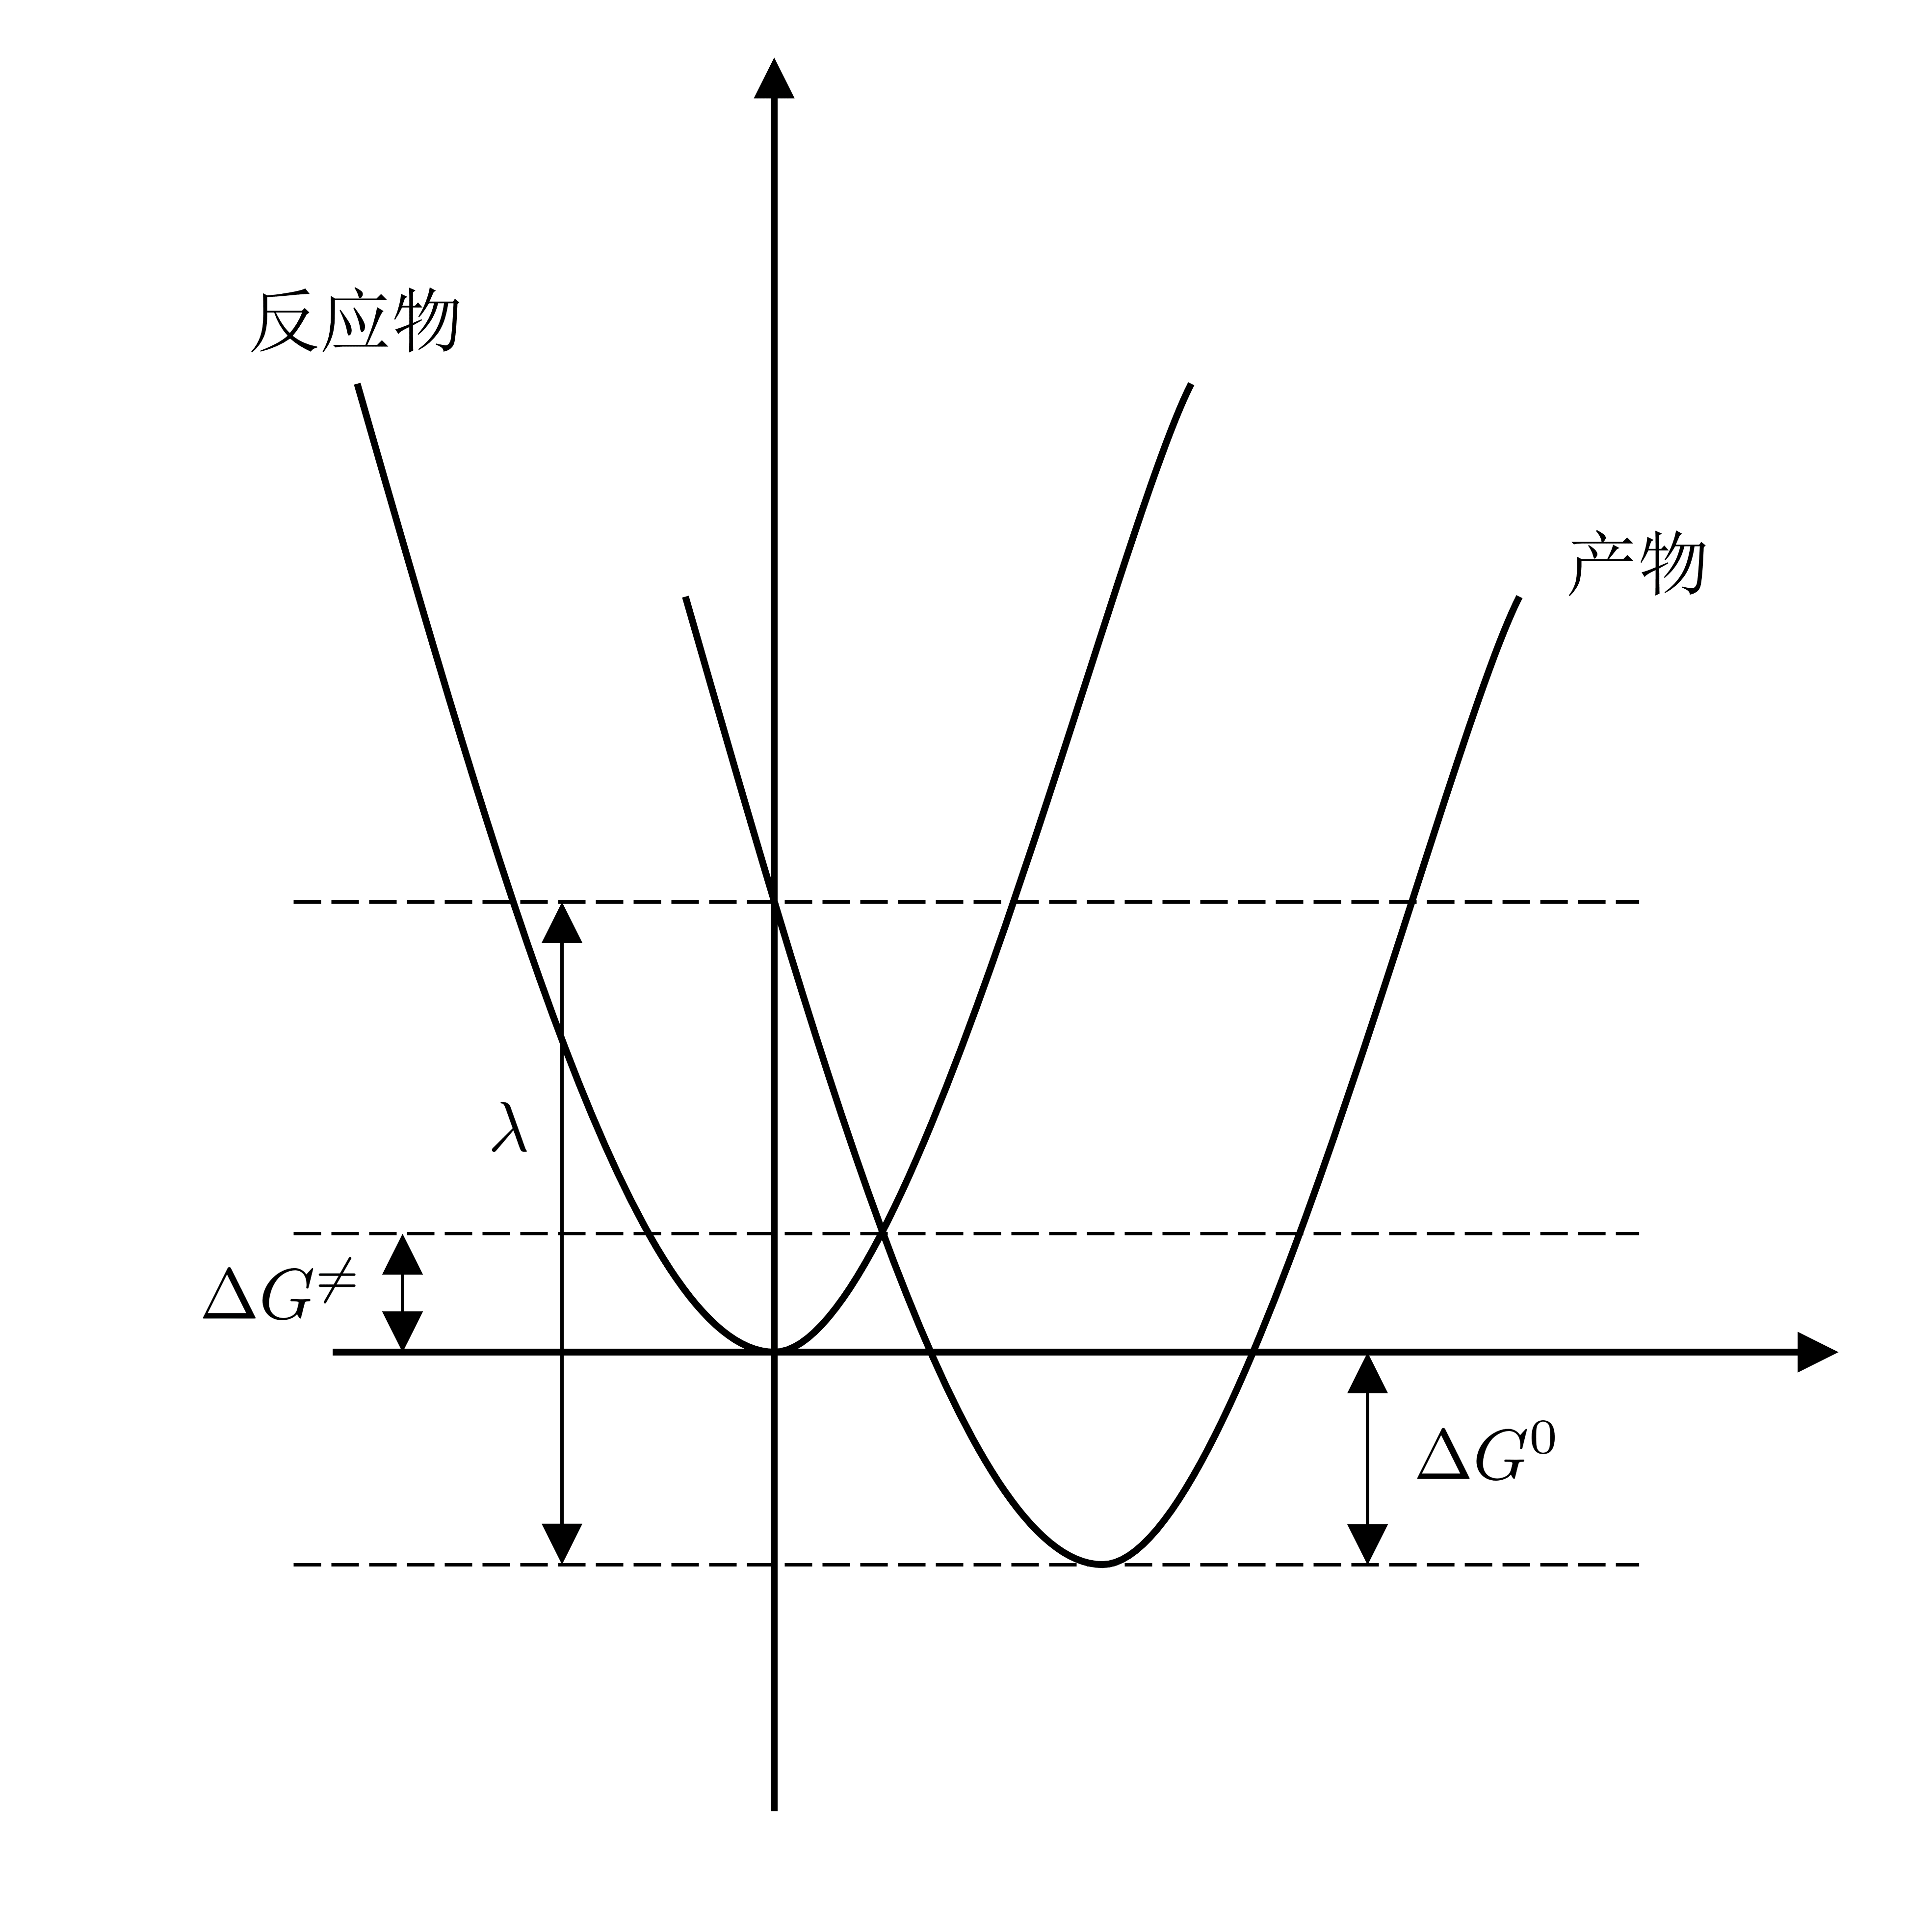
\includegraphics[width=0.5\textwidth]{re.png}
    \caption{重整能的计算示意图}\label{fig:re}
    \vspace{2mm}
\end{figure}

\chapter{结果与讨论}

%\chapter*{结\quad 论}
\chapter{总结与展望}

总结

%%%%%%%%%%  参考文献  %%%%%%%%%%
\defaultfont
\bibliographystyle{references/ref.buk}
\phantomsection
\markboth{参考文献}{参考文献}
\addcontentsline{toc}{chapter}{参考文献}       % 参考文献加入到中文目录
\nocite{*}                                     % 若将此命令屏蔽掉,则未引用的文献不会出现在文后的参考文献中
\bibliography{references/reference}
\titleformat{\chapter}{\centering\xiaosan\hei}{\centering\chaptername}{2em}{}
% !Mode:: "TeX:UTF-8"

%\titlecontents{chapter}[2em]{\vspace{.5\baselineskip}\xiaosan\song}%
%             {\prechaptername\CJKnumber{\thecontentslabel}\postchaptername\qquad}{} %
%             {}             % 设置该选项为空是为了不让目录中显示页码
\addcontentsline{toc}{chapter}{附\quad 录}
%\setcounter{page}{1}       % 如果需要从该页开始从 1 开始编页,则取消该注释
\markboth{附\quad 录}{附\quad 录}
\chapter*{附\quad 录}

\section*{附录A\quad OFET}

%% !Mode:: "TeX:UTF-8"

\titlecontents{chapter}[2em]{\vspace{.5\baselineskip}\xiaosan\song}%
             {\prechaptername\CJKnumber{\thecontentslabel}\postchaptername\qquad}{} %
             {}             % 设置该选项为空是为了不让目录中显示页码
\addcontentsline{toc}{chapter}{外文资料}
%\setcounter{page}{1}       % 如果需要从该页开始从 1 开始编页,则取消该注释
\markboth{外文资料}{外文资料}
\chapter*{外文资料}

Here follows the English paper.

...              % 外文资料
%% !Mode:: "TeX:UTF-8"

\titlecontents{chapter}[2em]{\vspace{.5\baselineskip}\xiaosan\song}
             {\prechaptername\CJKnumber{\thecontentslabel}\postchaptername\qquad}{}
             {}             % 设置该选项为空是为了不让目录中显示页码
%\addcontentsline{toc}{chapter}{中文译文}
%\setcounter{page}{1}            % 单独从 1 开始编页码
%\markboth{中文译文}{中文译文}   % 用于将章节号添加到页眉中
\chapter*{中文译文}

这里就是外文资料的中文翻译。

...
              % 中文译文,正常需被注释掉
% !Mode:: "TeX:UTF-8"

%\titlecontents{chapter}[2em]{\vspace{.1\baselineskip}\sihao\song}
%             {\prechaptername\CJKnumber{\thecontentslabel}\postchaptername\qquad}{} 
%             {}                            % 设置该选项为空是为了不让目录中显示页码
\fancypagestyle{plain}   % 设置页眉页脚风格,按照教务处规定,此处出现页眉,但是没有页脚(页码)。
\lhead{}
\rhead{}
\chead{\song\wuhao 天津大学 2024 届本科生毕业论文} % 设置页眉内容
\lfoot{}
\cfoot{}
\rfoot{}
\markboth{致\quad 谢}{致\quad 谢}
\addcontentsline{toc}{chapter}{致\quad 谢} % 添加到目录中
\chapter*{致\quad 谢}
%\setcounter{page}{1}

谢谢大家。            % 致谢
\clearpage
\end{document}                                 % 结束全文
